\documentclass[12pt]{article}
\usepackage[a4paper, margin=2cm]{geometry}
\usepackage{titlesec}
\usepackage{setspace}
\usepackage{amsmath}

% for tables
\usepackage{array}
\usepackage{booktabs}

% package that forces LaTeX to place an image in the exact position as it determied in the code
\usepackage{float} 

% for a rectangular box
\usepackage[most]{tcolorbox}

% package for multiple columns
\usepackage{multicol}
\setlength{\columnsep}{0.8cm} % separation between columns

\usepackage[utf8]{inputenc}

\usepackage{graphicx}
\usepackage{xcolor}

% For rotating figures, tables, etc. including their captions
\usepackage{rotating}

% small font size in the captions
\usepackage[font=small]{caption}

% header
\usepackage{fancyhdr}
\setlength{\headheight}{15.0pt}
\usepackage{ifthen}
\pagestyle{fancy}
\fancyhf{}
\fancyhead[L]{\ifthenelse{\value{page}=1}{}{Lessons \& Tutorials in Theoretical Chemistry}}
\fancyhead[R]{\ifthenelse{\value{page}=1}{}{Homework}}
\fancyfoot[C]{\thepage}

% bibliography
\usepackage[numbers]{natbib}
\bibliographystyle{unsrtnat}
\usepackage[colorlinks=true, linkcolor=blue, citecolor=blue, urlcolor=blue]{hyperref}
\renewcommand{\bibfont}{\small} % small font in the bibliography

% For DOIs in references
\usepackage{doi}
\renewcommand{\doitext}{DOI: }


\title{Quantum Dynamics - Homework}
\author{Albert Makhmudov}
\date{14/03/2025}

\begin{document}

\maketitle

\section*{Data Availability}
The source code of this project as well as the example input files are available at the corresponding \href{https://github.com/almakhmudov/LTTC-Homework--QD}{Github page}. There one could also find the example output files and the detailed instructions on how to run and compile the code. The example output files are \texttt{gif} animations of the wavepacket propagation that complement the results in \autoref{fig:snapshots}.

\section*{Code Overview}

% \begin{figure}[t!]
%     \centering
%     \includegraphics[width=0.9\textwidth]{deepmd.jpg}
%     \caption{The architecture of the \texttt{DeePMD} neural network potential. This figure has been reproduced from \citep{deepmd2024gomez}.}
%     {\color{gray}\rule{\linewidth}{0.1mm}}
%     \label{fig:deepmd}
% \end{figure}

\begin{sidewaysfigure}[ht]
    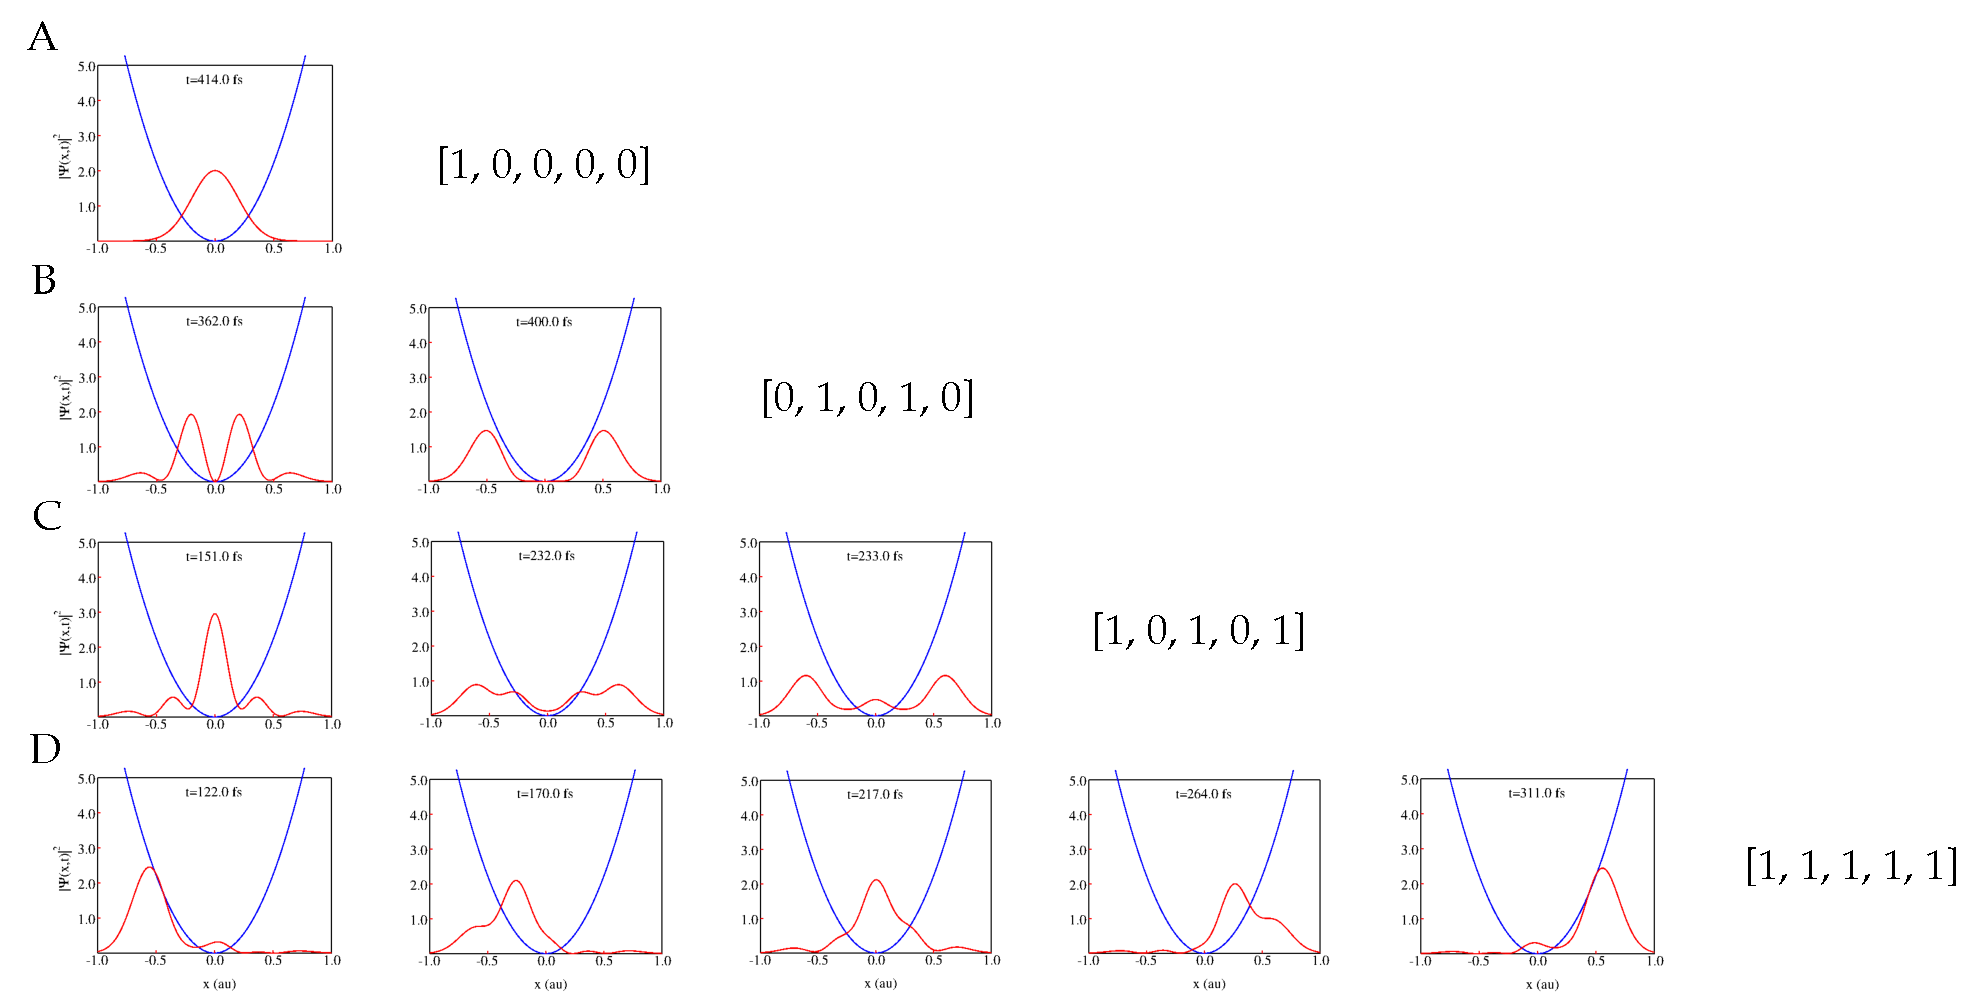
\includegraphics[width=\textwidth]{snapshots.pdf}
    \caption{Time evolution of the wavepackets with different number of eigenstates. The wavepackets were propagated using the \textbf{(A)} $[1, 0, 0, 0, 0]$, \textbf{(B)} $[0, 1, 0, 1, 0]$, \textbf{(C)} $[1, 0, 1, 0, 1]$, and \textbf{(D)} $[1, 1, 1, 1, 1]$ coefficients.}
    \label{fig:snapshots}
\end{sidewaysfigure}

\section*{Results and Discussion}

% \begin{figure}[t!]
%     \centering
%     \includegraphics[width=1.0\textwidth]{forces_correlation_plot.png}
%     \caption{Correlation between predicted and reference forces. The predictions were obtained from the NNPs trained on 500 configurations but with different number of iterations, e.g. \textbf{(A)} 500, \textbf{(B)} 50000, \textbf{(C)} 600000.}
%     {\color{gray}\rule{\linewidth}{0.1mm}}
%     \label{fig:forces_correlation}
% \end{figure} 

\section*{Generative AI Usage}
In this work, \href{https://chatgpt.com}{ChatGPT} large language model was used to check grammar and spelling of the main body of text, whilst \href{https://www.perplexity.ai}{Perplexity} was utilized for the sake of literature search.

\section*{Acknowledgments}
This project is based on data and instructions provided by Arjan Berger available at the aforementioned \href{https://github.com/almakhmudov/LTTC-Homework--QD}{Github page}.

\bibliography{references}

\end{document}